\section{Wired Equivalent Protocol - WEP}


\ac{WEP} is a security protocol, defined in \ac{IEEE}802.11, to secure link-level data throughout wireless transmission. Its message encryption and decryption mechanism was aimed to provide three main goals: confidentiality, access control and data integrity from data-link layer.
\subsection{WEP mechanism}\label{subsec:wep_mec}
\ac{WEP} mechanism is based on the \ac{RC4} algorithm\cite{mousa2006evaluation} that aims to supply security to \ac{WLAN} equivalent to \ac{LAN}. In general, the \ac{WEP} encryption of a frame includes three steps described in details in \ac{IEEE}802.11 standard \cite{al2006ieee}. The encryption algorithm takes input as a plaintext $M$ and produce the output $C$ and transmit over the network. The three steps of \ac{WEP} would be described as below
\begin{steps}
	\item \ac{WEP} calculates checksum $c(M)$ and concatenate with the original plaintext $M$, we have the message $P = <M, c(M)>$
	\item \ac{WEP} would encrypt the message $P$ achieved in the first step using \ac{RC4}. \ac{RC4} generates a keystream relying on the \ac{IV} $v$ and a key $k$. The keystream is denoted as $RC4(v,k)$. We use \ac{Xor}on the plain text and key stream to get the output $C$ of this step is $C = P \oplus RC4(v,k)$
	\item Concatenate $C$ achieved in step 2 with the \ac{IV} and transmit $<C, v>$ over the network.
\end{steps}

An \ac{AP} would catch the message and decrypt it by using \ac{Xor} operation over the encrypted message with \ac{RC4} key stream.  First, \ac{WEP} would extract message in to $v$ and $C$. After that, a \ac{RC4} keystream would be generated and \ac{Xor} it against $C$ to obtain plaintext $P$:
\begin{center}
	\begin{align}
	P'&= C \oplus RC4(v, k) \\
	&= (P \oplus RC4(v, k)) \oplus RC4(v, k) \\
	&= P
	\end{align}
\end{center}

	
$P$ includes $M$ and checksum $c(M)$. The receiver would split $P$ and check if the checksum is matched or not. The whole protocol of \ac{WEP} is described in \autoref{fig:wep}
\begin{figure}
	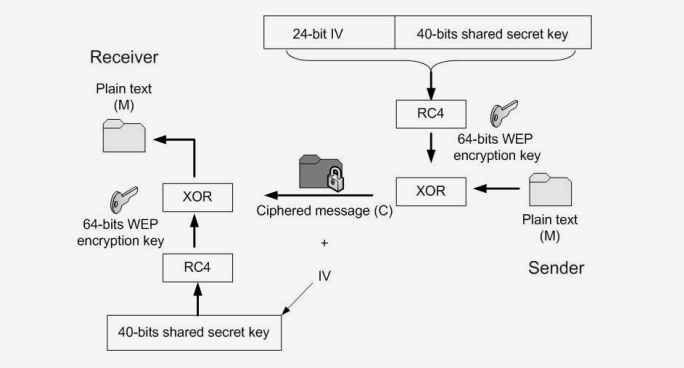
\includegraphics[scale=0.35]{images/wep.png}
	\caption{The WEP protocol \cite{al2006ieee}}
	\label{fig:wep}
\end{figure}

\subsection{Keystream reuse attack}

The main problem of \ac{WEP} is the length of secret key. As the length of shared secrete key is $40bits$, the possibility of reusing this secret key is extremely high \cite{al2006ieee}. Although \ac{RC4} algorithm can support the length of the secret key up to $104bits$, it would be infeasible to stop attackers to explore the key in less than 15 minutes \cite{convery2003cisco}. Furthermore, the use of shared secret key which is higher than $40bits$ might causes communication problems as the default setting on other devices is $40bits$. 

The use of $24bits$ \ac{IV} is another problem. the number of possible \ac{IV} is $2^{24}$. This is a small number in the scope of data transmission which causes multiple uses of \ac{IV}. The reuse of \ac{IV} is often called "\ac{IV} collision". Moreover, the transmission of \ac{IV} is clear over the network, it would deteriorate the weakness of \ac{WEP}. Moreover, \citeauthor{shunman2003wlan} in \cite{shunman2003wlan} describe several security problems of using \ac{RC4} keystream. \ac{RC4} does not support random access which is a fatal pitfall in security of \ac{WEP} as it make the crypt-analysation effort-less.

This \ac{WEP} scheme would cause a serious problem if two cipher texts use the same \ac{RC4} key stream. Due to the \ac{Xor} operation properties, the \ac{Xor} operation over two ciphertext using the same key stream will result equivalent to the \ac{Xor} operation over two corresponding plaintexts:

\begin{align}
	C_1 &= P_1 \oplus RC4(v,k)\\
	C_2 &= P_2 \oplus RC4(v,k) \\
	C_1 \oplus C_2 &= (P_1 \oplus RC4(v,k)) \oplus (P_2 \oplus RC4(v,k))\\
	C_1 \oplus C_2 &= P_1 \oplus P_2
\end{align}

The above peril property of \ac{RC4} might incapacitate most of the security goals in \ac{WLAN} as the attacker might know $P_1$ or $P_2$ and do the \ac{Xor} operation again to get the original plaintext of others. This means that any adversary who know a plaintext can use it to decrypt others. As a result, In case that an adversary obtains these two conditions:
\begin{itemize}
	\item Ciphertexts that use the same keystreams.
	\item The availability of several plaintexts.
\end{itemize}
he or she would negate all the efforts of \ac{WEP} to provide confidentiality  outrageously. Unfortunately, both of the above conditions could absolutely be achieved by skillful and patient attackers.


\subsubsection{Keystream duplication detection}~\\
\citeauthor{borisov2001intercepting} in \cite{borisov2001intercepting} discuss several flaws in design of WEP that an adversary can exploit to achieve keystream reuse. 

First, \ac{IV}'s are public, so any reuse of \ac{IV}'s might be easily detected. An adversary, who is able to detect duplicate \ac{IV}'s, might collect a large number of sets of the same keystream ciphertexts. 

Second, the \ac{PCMCIA} standard mechanism is another issue. The \ac{PCMCIA} normally resets \ac{IV} $v$ to $0$ every time \ac{PCMCIA} is re-initialized, after that increments by $1$ for each packet transmission. Consequently, keystreams, corresponding to low-valued \ac{IV}'s, seems to be reused more frequently. 

Finally, \ac{WEP} standard exposes all \ac{WEP} implementation. This often leads to serious risks of keystreams exposure. As the duplication of \ac{IV} is unavoidable in \ac{WEP}, a patient attacker would readily get a duplicate \ac{IV} whenever it appears. Due to \ac{WEP} mechanism, this issue can not be thwarted.

In conclusion, there are many security holes in the architecture of \ac{WEP} that an adversary can exploit to detect keystream reuse. Through network observation, a patient attacker might have chance to acquire a large set of ciphertexts which have the same keystream.

\subsubsection{Plaintexts acquirement}~\\
Authors in \cite{borisov2001intercepting} also analyse about the risk of the plaintext availability to an adversary.

As above discussion, if one plaintext is known, it is easy to derive the contents of another directly. As a result, plaintext security is another threat to \ac{WLAN}

An attacker might derive the contents of several predictable messages. Login, an authenticated step familiar to Internet users, often has some password prompts or welcome message, which can be acquired by an adversary. Another example is that the attacker could analyse the traffic patterns and lengths. Those techniques would provide a large quantity of plaintexts feasible to keystream reuse attack.

Another technique is to cause the plaintext to be transmitted between devices under control of that attacker then observe the encrypted form and decrypted form of that plaintext. The attacker may also send spam e-mail to an user and wait for them to check over wireless link. This method is considered thoughtful as it does not raise too many alarms.

In some circumstances, plaintext obtaining seems to be simpler. As the attacker would actively observe the encrypted from and decrypted form of messages over network. As \ac{STA} broadcasts the messages to all \ac{AP}, this problem is unavoidable.

\subsubsection{Decryptional Dictionaries}~\\
Once the plaintext of a ciphertext is obtained, the attacker would probe the value of keystream used in that ciphertext. Overtime, he or she could build a table of the keystream corresponding to each \ac{IV} as well as plaintext. The complete table might encroach $24GB$ external memory and it would help the attacker to immediately decrypt each ciphertext in \ac{WLAN} with very little work. In \cite{al2006ieee}, \citeauthor{al2006ieee} call this attack is "dictionary attack".


\subsection{Message Authentication}
Another provision of \ac{WEP} is message authentication through Integrity checksum. The Integrity checksum is utilised to ensure that the message is not modified. It is implemented as a \ac{CRC} variant (\ac{CRC}-32), a piece of the packet decrypted payload.

However, the protection of \ac{CRC} is not sufficient to protect message from modification. it is designed to check if an error appears in the message, yet it is not resistant to malicious attacks. Once again, the \ac{WEP} protocol use stream cipher exacerbates the vulnerability of \ac{CRC}.

\subsubsection{Message Modification}
\newtheorem{property}{Property}

\begin{property}
	\ac{WEP}'s checksum is a linear function of the message
	\label{prop:linear}
\end{property}

The Property \autoref{prop:linear} reveals that checksumming function distributes over \ac{Xor} operations.
\begin{equation}
	c(a\oplus b) = c(a) \oplus c(b)\, \forall a,b
	\label{equation:linear_prop}
\end{equation}

As a consequence, the process of modifying ciphertexts without intervening the checksum become possible. In \autoref{subsec:wep_mec}, we describe the final step of sending message in \ac{WEP}:
\begin{equation}
	A \rightarrow B : <v,C>
\end{equation}
While $C$ is ciphertext $C = RC4(v,k) \oplus <M, c(M)>$ and $v$ is $IV$. We would describe the technique below to turn a transmitted message $<v, C>$ into $<v, C'>$ in which $C'$ decrypts $M'$. $M'$ is modified message of $M$ by using \ac{Xor} operation $M' = M\oplus \Delta$ in which $\Delta$ is chosen arbitrarily.
